
%%%%%%%%%%%%%%%%%%%% author.tex %%%%%%%%%%%%%%%%%%%%%%%%%%%%%%%%%%%
%
% sample root file for your "contribution" to a contributed volume
%
% Use this file as a template for your own input.
%
%%%%%%%%%%%%%%%% Springer %%%%%%%%%%%%%%%%%%%%%%%%%%%%%%%%%%


% RECOMMENDED %%%%%%%%%%%%%%%%%%%%%%%%%%%%%%%%%%%%%%%%%%%%%%%%%%%
\documentclass[graybox]{svmult}

% choose options for [] as required from the list
% in the Reference Guide

\usepackage{mathptmx}       % selects Times Roman as basic font
\usepackage{helvet}         % selects Helvetica as sans-serif font
\usepackage{courier}        % selects Courier as typewriter font
\usepackage{type1cm}        % activate if the above 3 fonts are
                            % not available on your system
%
\usepackage{makeidx}         % allows index generation
\usepackage{graphicx}        % standard LaTeX graphics tool
                             % when including figure files
\usepackage{multicol}        % used for the two-column index
\usepackage[bottom]{footmisc}% places footnotes at page bottom
\usepackage{marginnote}
\newcommand{\TODO}[1]{\marginnote{TODO: #1}}    % TODO Befehl
\usepackage{units,subfigure,amsmath}
\usepackage{wrapfig}
\usepackage{todonotes}
\usepackage{hyperref}
\hypersetup{
    colorlinks=true,
    linkcolor=blue,
    filecolor=magenta,      
    urlcolor=cyan,
}
\usepackage{url}
% see the list of further useful packages
% in the Reference Guide

\makeindex             % used for the subject index
                       % please use the style svind.ist with
                       % your makeindex program

%\usepackage{cleveref}[2012/02/15]
%\crefformat{footnote}{#2\footnotemark[#1]#3}

\renewcommand{\O}{{\cal O}}
\renewcommand{\leadsto}{\rightsquigarrow}
\newcommand{\V}[1]{\text{\boldmath $#1$}}    % Format for "Vector"
\newcommand{\M}[1]{\V{#1}}                   % Format for "Matrix"

\newcommand{\R}{\mathbbm{R}}                 % set of real number
\newcommand{\N}{\mathbbm{N}}                 % set of natural numbers
\newcommand{\C}{\mathbbm{C}}                 % ...
\newcommand{\1}{\mathbbm{1}}                 % identity matrix


%%%%%%%%%%%%%%%%%%%%%%%%%%%%%%%%%%%%%%%%%%%%%%%%%%%%%%%%%%%%%%%%%%%%%%%%%%%%%%%%%%%%%%%%%

%%
% Motivation, Problem Statement, Related Work (one page)
% Technical Approach (one page)
% Results (one page)
% Experiments completed or scheduled (one page)
% Main experimental insights (one page)
% References (one page)
%%

\begin{document}

\title*{L.U.N.A. - A Laser-Mapping Unidirectional Navigation Actuator} 
\author{Jasper Zevering, Anton Bredenbeck, Fabian Arzberger,
  Dorit Borrmann and Andreas N\"uchter}
% FIXME sort the authors
% Use \authorrunning{Short Title} for an abbreviated version of
% your contribution title if the original one is too long
\institute{All authors are with Informatics VII -- Robotics and
  Telematics, University of W\"urzburg, Am Hubland, 97074 W\"urzburg
  \email{borrmann@informatik.uni-wuerzburg.de} \\|  \email{jasper.zevering@stud-mail.uni-wuerzburg.de} \\ | \email{anton.bredenbeck@stud-mail.uni-wuerzburg.de}\\ |  \email{fabian.arzberger@stud-mail.uni-wuerzburg.de}
%\and Name of Second Author \at Name, Address of Institute 
%\email{name@email.address}
}
%
% Use the package "url.sty" to avoid
% problems with special characters
% used in your e-mail or web address
%
\maketitle

%\abstract*{Each chapter should be preceded by an abstract (10--15 lines long) 
%that summarizes the content. The abstract will appear \textit{online} at 
%\url{www.SpringerLink.com} and be available with unrestricted access. This 
%allows unregistered users to read the abstract as a teaser for the complete 
%chapter. As a general rule the abstracts will not appear in the printed 
%version 
%of your book unless it is the style of your particular book or that of the 
%series to which your book belongs.
%Please use the 'starred' version of the new Springer \texttt{abstract} command 
%for typesetting the text of the online abstracts (cf. source file of this 
%chapter template \texttt{abstract}) and include them with the source files of 
%your manuscript. Use the plain \texttt{abstract} command if the abstract is 
%also to appear in the printed version of the book.}
\abstract{
The abstract goes here.
README: Feel free to change and cut content as you see fit! I've written down everything that came to my mind fairly independent of its quality. - A.
}

\section{Introduction}
\label{sec:introduction}

In today's world, autonomous robots have found their way into everyday life in a variety of ways. This includes, but isn't limited to, the vacuum cleaner that independently navigates one's living-room or mobile robots employed for exploration of areas that are too dangerous for humans. To foster new advances in the latter, specifically for underground environments, the  Defense Advanced Research Projects Agency (DARPA) of the US Defense Department established the yearly "SubT" Challenge in 2017. In this challenge, teams are tasked to "Drive novel approaches and technologies to allow warfighters and first-responders to rapidly map, navigate, and search dynamic underground environments."  \cite{allen} proving the demand for further research in this domain. One difficulty of this challenge is building an accurate 3D model of the environment, i.e. mapping the surroundings. The teams that participate in the DARPA challenge take advantage of high-quality hardware, such as state-of-the-art 3D laser-scanners and cameras, thus making their solutions rather expensive. However, the demand for mapping-solutions in the low-cost sector is non-negligible. 

\todo[inline]{Previous low cost 3D laser scanning approaches.I'm unhappy with the complete next paragraph. From here...}
"Classical Mechanics Scanner" \cite{classical_mechanics_scanner}

Previous work was also done at the Julius-Maximilians University W\"urzburg \cite{ISER2018}. The RADLER (RADial LasER scanning device) consists of a 2D laser scanner attached to the axle of a unicycle. An operator then pushes the unicycle along a requested path. The inherent rotation of the wheel then creates a radial 3D laser-scanning pattern. However, this approach still requires an operator, therefore does not fulfill the autonomy requirements. 

A more autonomous approach was taken in \cite{3D_per_2D_based}. The authors mounted a rotating 2D laser-scanner on top of a \href{https://www.turtlebot.com}{turtle-bot} thus removing the need of an operator. In contrast to the RADLER however, does the turtle-bot not provide an inherent rotation. Therefore an extra actuator is required to create the radial 3D scanning-pattern. \todo[inline]{...to here}

Building upon the results of the RADLER  this paper presents a novel approach to low-cost 3D laser-scanning using a 2D laser-scanner inside a torque driven spherical robot: the L.U.N.A. - sphere (Laser-mapping Unidirectional Navigation Actuator). The 2D laser-scanner is fixed to the spherical structure, hence a similar situation as with the RADLER is given: the inherent rotation of the sphere creates a radial 3D scanning pattern. 


\section{State of the Art}
\label{sec:stateOfTheArt}
As evolution of RADLER as hand-driven radial scanner device, a self-driving spherical approach was chosen to ensure robustness and autonomy.  There have been several works in literature regarding approaches for spherical robots as well as 3D scanning mechanisms. 

\subsection{Spherical Robots}
\label{sec:stateOfTheArt:sphericalrobots}
An early idea of an self-driving sphere has been introduced by J.L. Tate in 1893 who claimed the patent  508 and 558 in  the U.S. for a sphere, driven by an inner moving counterweight, which got its torque from an spring. This idea of an actuator attached to an counterweight pointing to the bottom and therefore the torque being transferred to the sphere and moving it, is still a wide spread approach for spherical robots.

In \cite{soa1} a basic motion controll system for the BYQ-III is introduced. The BYQ-III has a mass of 25kg and a diameter of 600mm and its diving mechnaism has been proposed in \cite{soa2} by S.Hanxu, X,Aiping, J.Qingxuan and W.Liangqing. It contains  a counterweight pendulum, four gyros providing movement for two axes and one IMU mounted on the gyro case. There is no extra payload or Sensor, nor would there be space for a centered measurement unit due to the centered counterweight. Therefore the counterweight leads to a steady movement no relying on acceleration but on velocity of the actuators and therefore providing continuous speed.

A second spherical robot with its driving mechanism relaying on inner counterweight is preented in \cite{soa3}. This was designed for movement on water-surface and therefore having orthogonal to the movement mounted fins on the shell. Two actuators attached to the shell and the inner counterweight provide movement around one axis. In contrast to the BYQ-III a middle-centered  sensor would be possible, but this would have no movement relative to the surface, as it would be part of the relatively non moving inner counterweight. It also has steady, well controllable movement. 
The sphere presented in \cite{soa4} \cite{soa5} provides an solution for a driving system which does not relay on a moving inner counterweight but uses internal reaction wheels to provide torque. This leads to theoretically having middle-centered space which is rolling an not steady steady to the environment.  But the prototype provided by Vijay Muralidharan shows less controllability then counterweight driven spheres. Also now it is driven by acceleration and not velocity which leads to limited movement.

A third approach for spherical robots relays on an internal unit which drives in the sphere. A Design and control approach is provided in \cite{soa6} where an four-wheeled vehicle moves in the sphere to force it rolling by moving the center of mass in the desired direction. This technical solution is capable of a nearly maximum size of possible payload in relation to the overall-size, but also does not  provide without further mechanics a rotation of the senser which would be needed for 3-dimensional laser scanning.Also this provides just like the counterweight driven approach a good controlability, it is obviously not as stable regarding external perturbations or forces, due to the missing fixed connection to the shell. This would make it not suitable for mission with extreme forces and unknown starting conditions like missions involving a rocket launch or an drop to the starting point, which would lead to harsh movements of the in the worst case a start with the unit being rotated 180 degree and therefore not being able to bring torque to the sphere. This would also happen if the sphere was stuck to to the environment and therefore the inner unit trying to perform a whole revolution of the sphere, which leads to a supine position.

Overcoming this shortage of the inner unit just relaying on gravity to apply its force to the shell, \cite{soa7} introduced the approach of a rod, expanded by a spring to the maximum possible size and having a wheel on one side. The wheel generates the movement by again moving the center of weight. But now the non-reversible supine position does not exist anymore, because even with the wheel being at the top, it still is pressed to the shell by the spring and therefore being able of maintaining its movement. Again this approach does not provide spin of a centered  placed sensor without further contraptions.



\subsection{3D Laser Scanning}
\label{sec:stateOfTheArt:3Dlaserscanning}

\todo[inline]{Talk about 3D laser scanning. Specifically on mobile robots}

\section{Technical Approach}
\label{sec:TechnicalApproach}

\begin{figure}
\centering
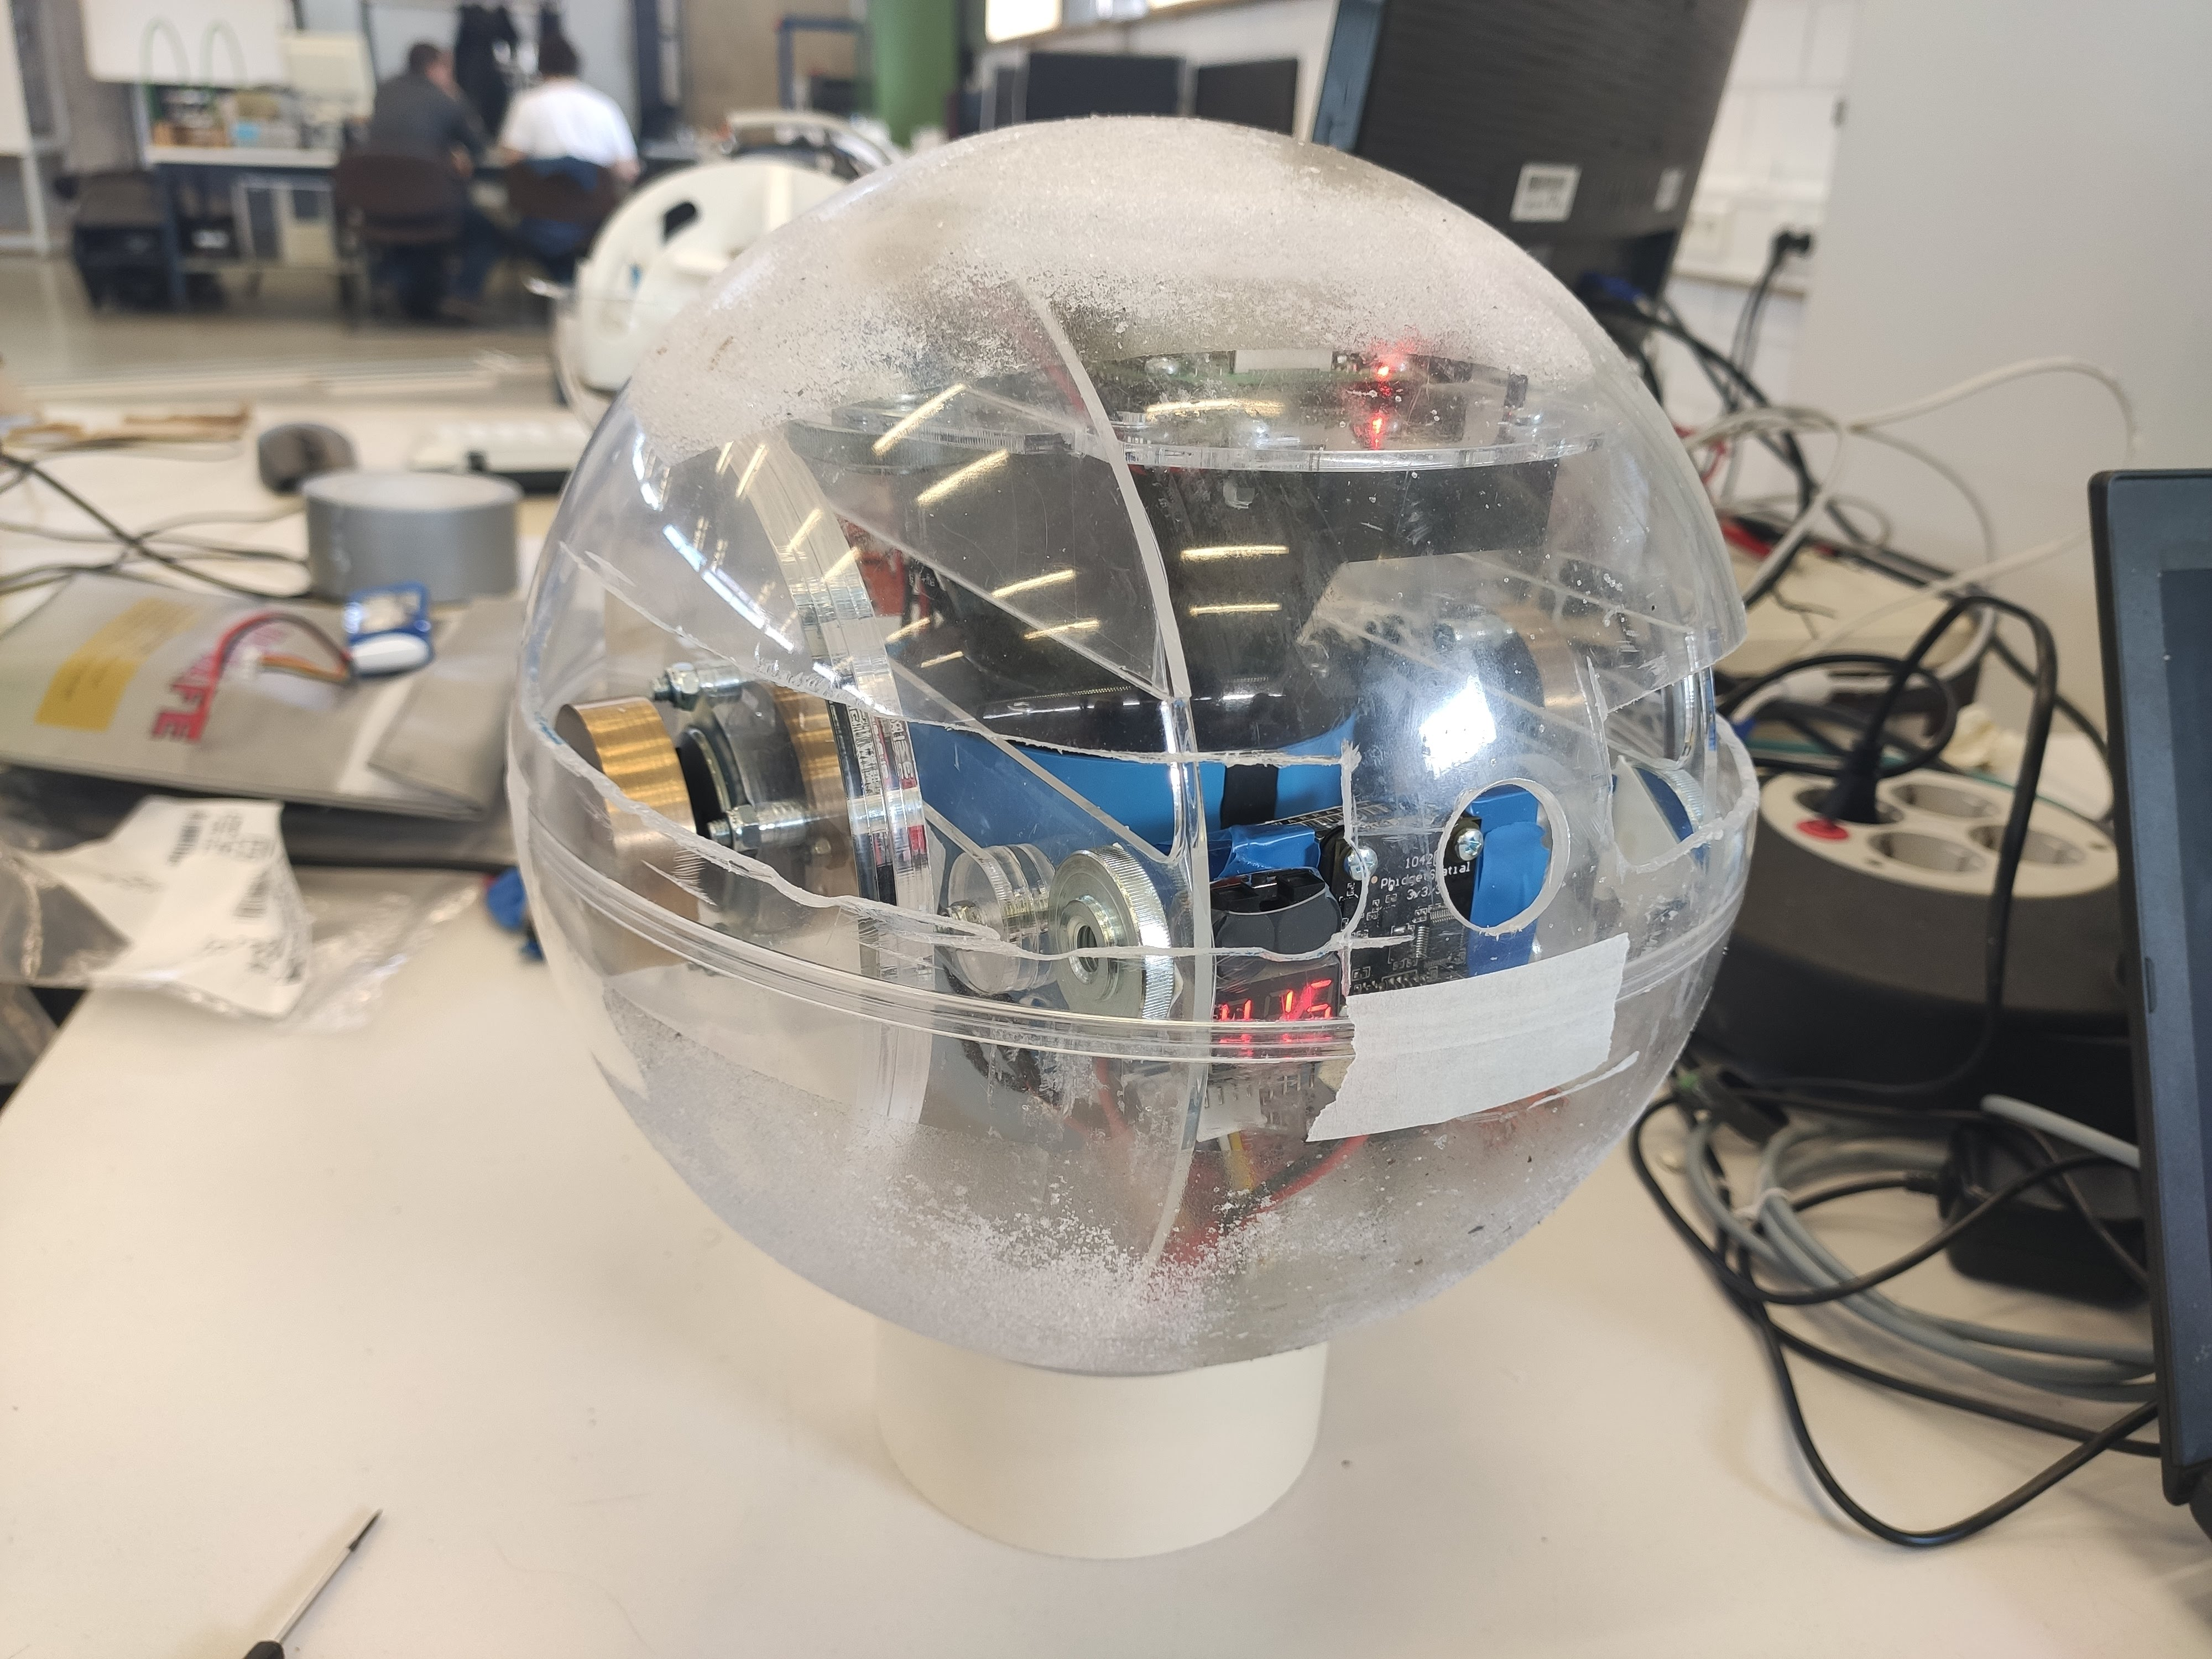
\includegraphics[height=50mm]{../Media/sphereFullshellLeft.jpg}
\hfill
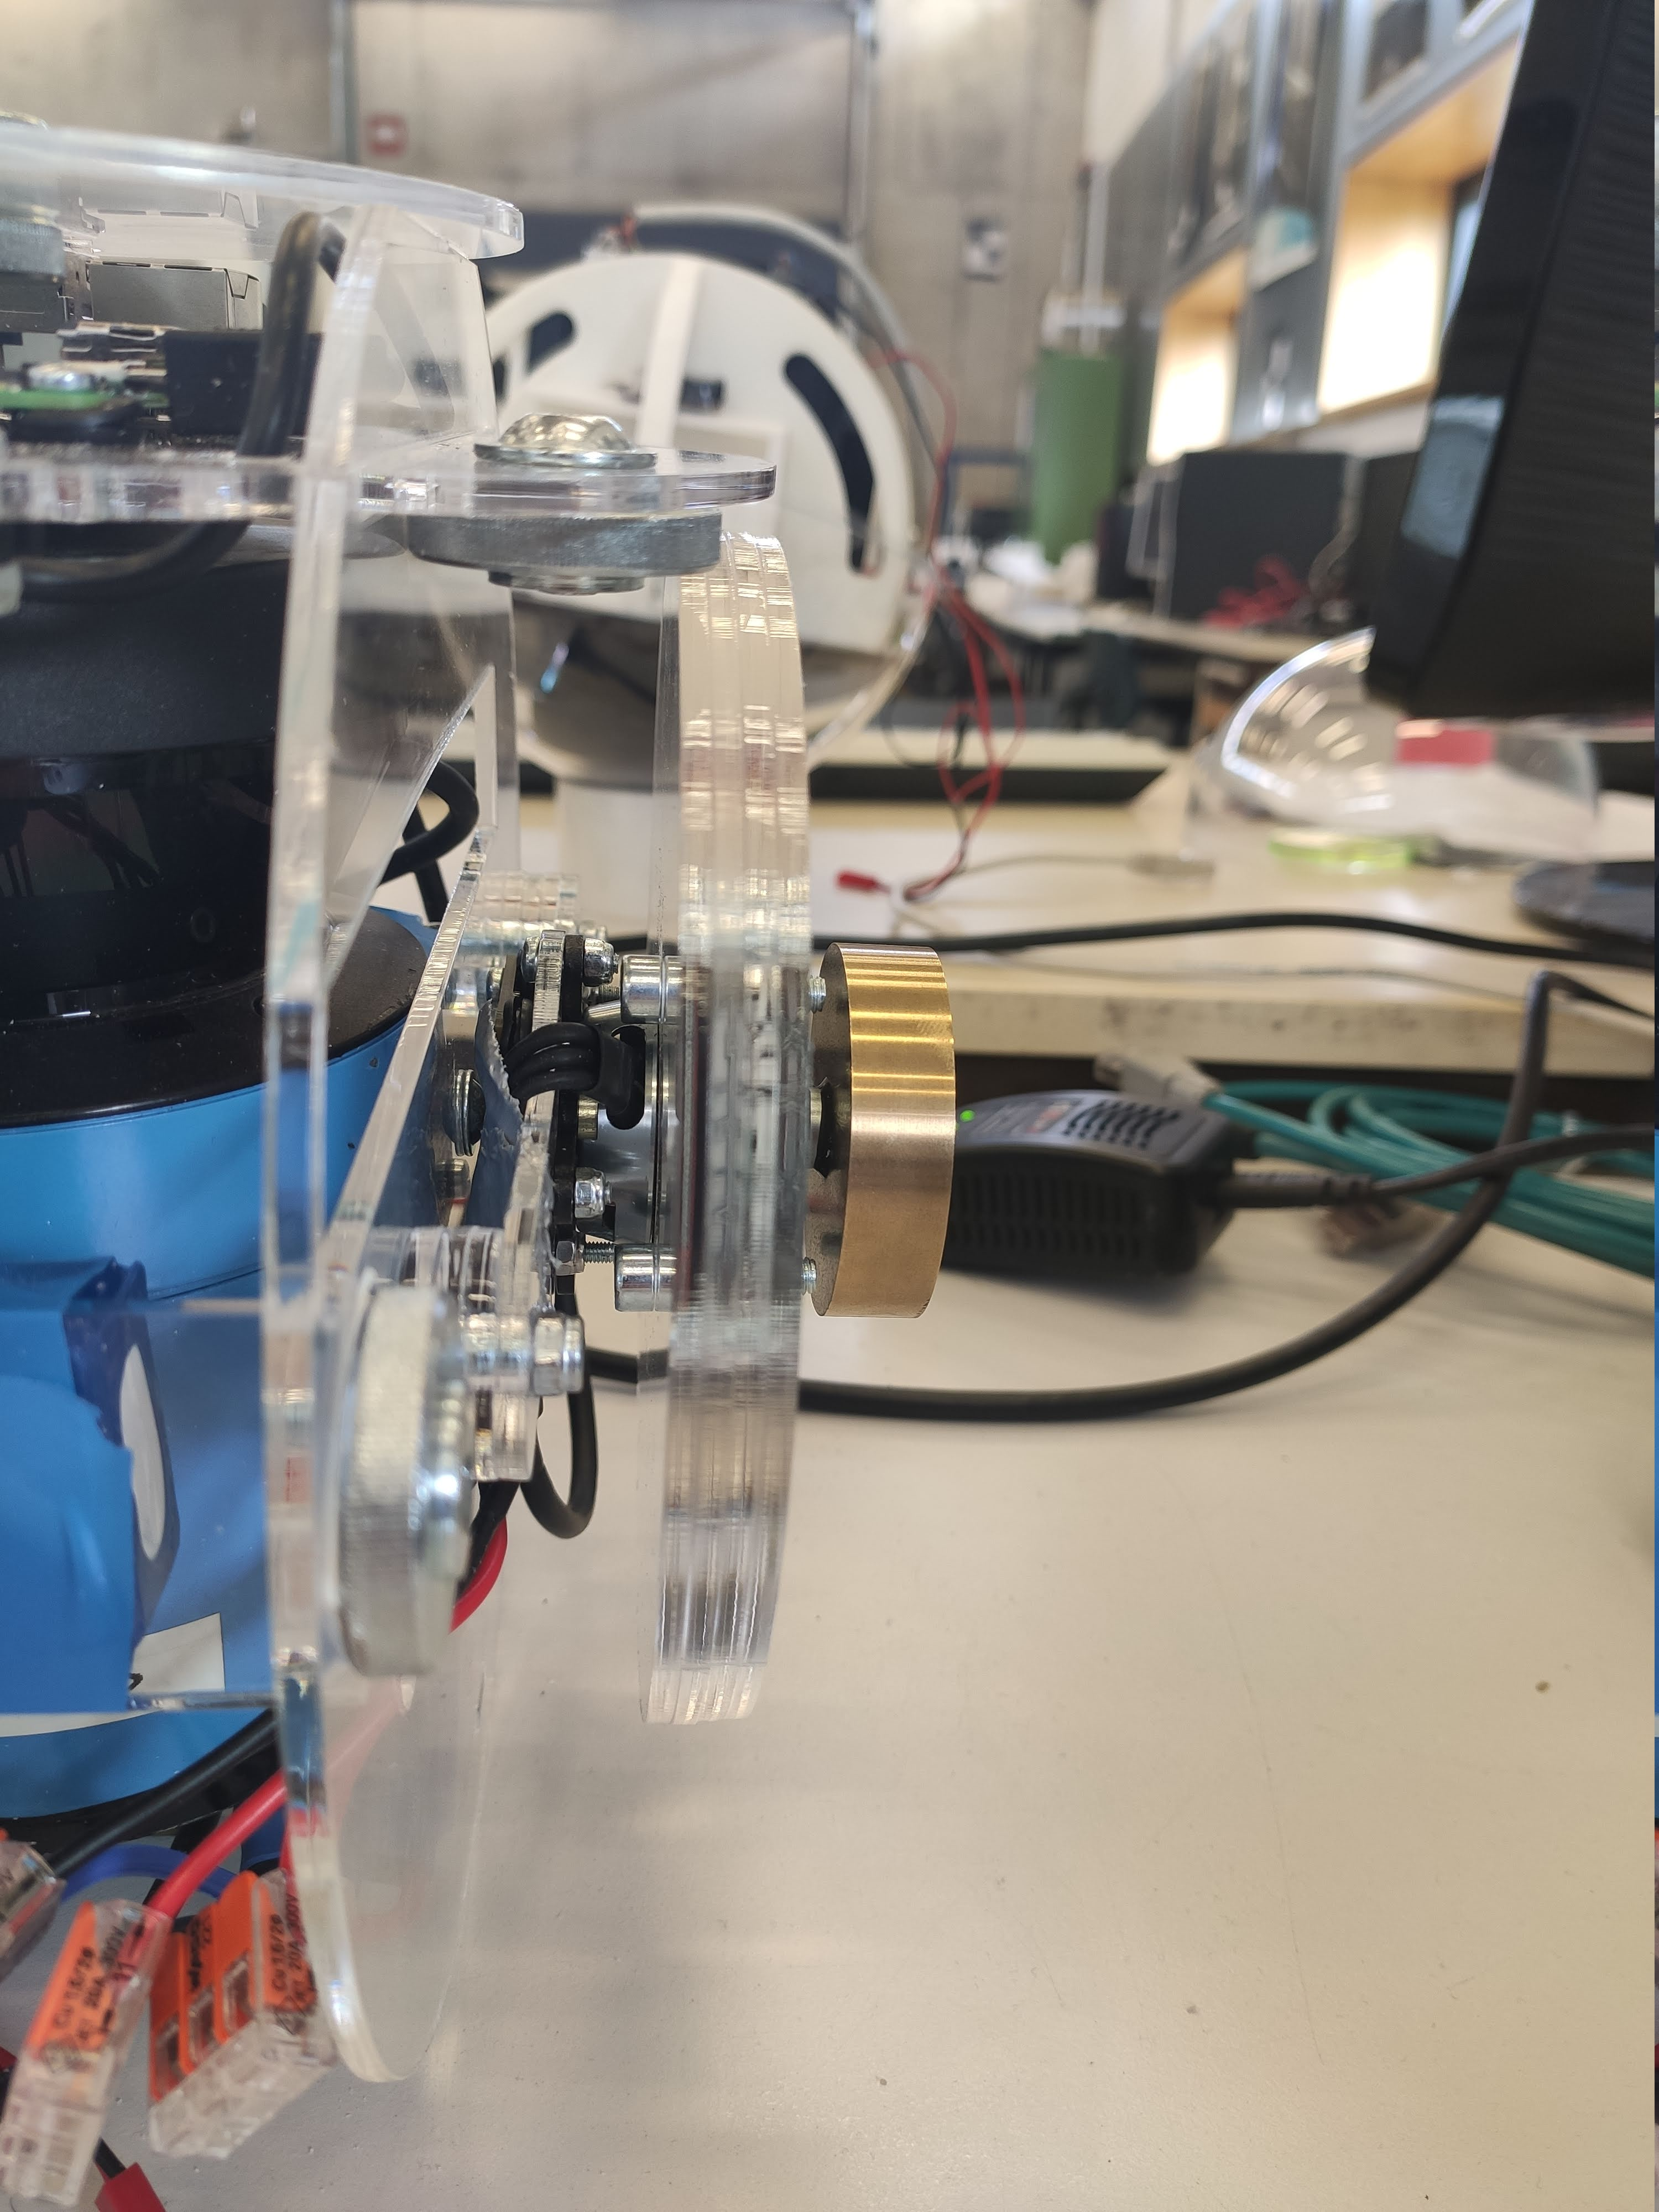
\includegraphics[height=50mm]{../Media/sphereRightMotor.jpg}   
\label{sec:TechnicalApproach:fig:motor}
\label{sec:TechnicalApproach:fig:prototype}
\caption{Hardware setup of the L.U.N.A sphere prototype, including notches in the shell and friction granule. IMU (beneath supporting structure) and brushless motor (above supporting structure) of the L.U.N.A sphere without shell, including flywheel mass. Hardware setup of the L.U.N.A sphere prototype, including notches in the shell and friction granule.}
\end{figure}

\todo{Bilder mit hoehe anpassen, keine captions in subfigures, optimale mm werte finden, caption anpassen (left / right) }

\todo{Wie dreht sich die Kugel überhaupt ? COAM + Cubli paper lesen / gyro effekt + video schneiden (ohne ton) }

Figure \ref{sec:TechnicalApproach:fig:prototype} shows the final hardware setup of the robot.
\todo{was ist da drinnen (raspberry pi, ..), wo ist es da drinnen, warum ist es da drinnen.}
In order to reduce complexity with respect to the 3D-transformation calculations, the laserscanner was placed at the center of a spherical acrylic glass shell as precisely as possible.
This limits the laser scanners movement to rotational movement and removes translational movement completely. With this initial setup given, the only room left for the acrylic glass structural components, batteries, boardcomputer, IMUs, motors, weights and wiring are the spaces between the scanner and the shell.
Figure \ref{sec:TechnicalApproach:fig:motor} shows one Turnigy Park480 brushless outrunner motor \cite{turnigymotor} of the COAM drive with two flywheels attached.
Strong epoxy glue attaches the weights to the motor shafts and shells.
As the flywheels start spinning with respect to the structural components of the sphere, the sphere itself starts spinning with respect to the ground. 

Figure \ref{sec:TechnicalApproach:fig:prototype} also shows that the top and the bottom of the shell are covered in table salt, which made a good granule to increase friction to the ground in the early testing phase. Furthermore, there are notches in the front side of the shell to increase permeability for the laser.
Unfortunately, the laser scanner measurements are still affected by blockades due to components of the sphere.
Specifically, the outside shell is an inhibiting factor as an object with the distance of the radius is measured at all times, \todo{which is why measurement slits}
                                                                                                                                                                                                                  
\begin{figure}                                                                                                                                                                                                    
\centering                                                                                                                                                                                                        
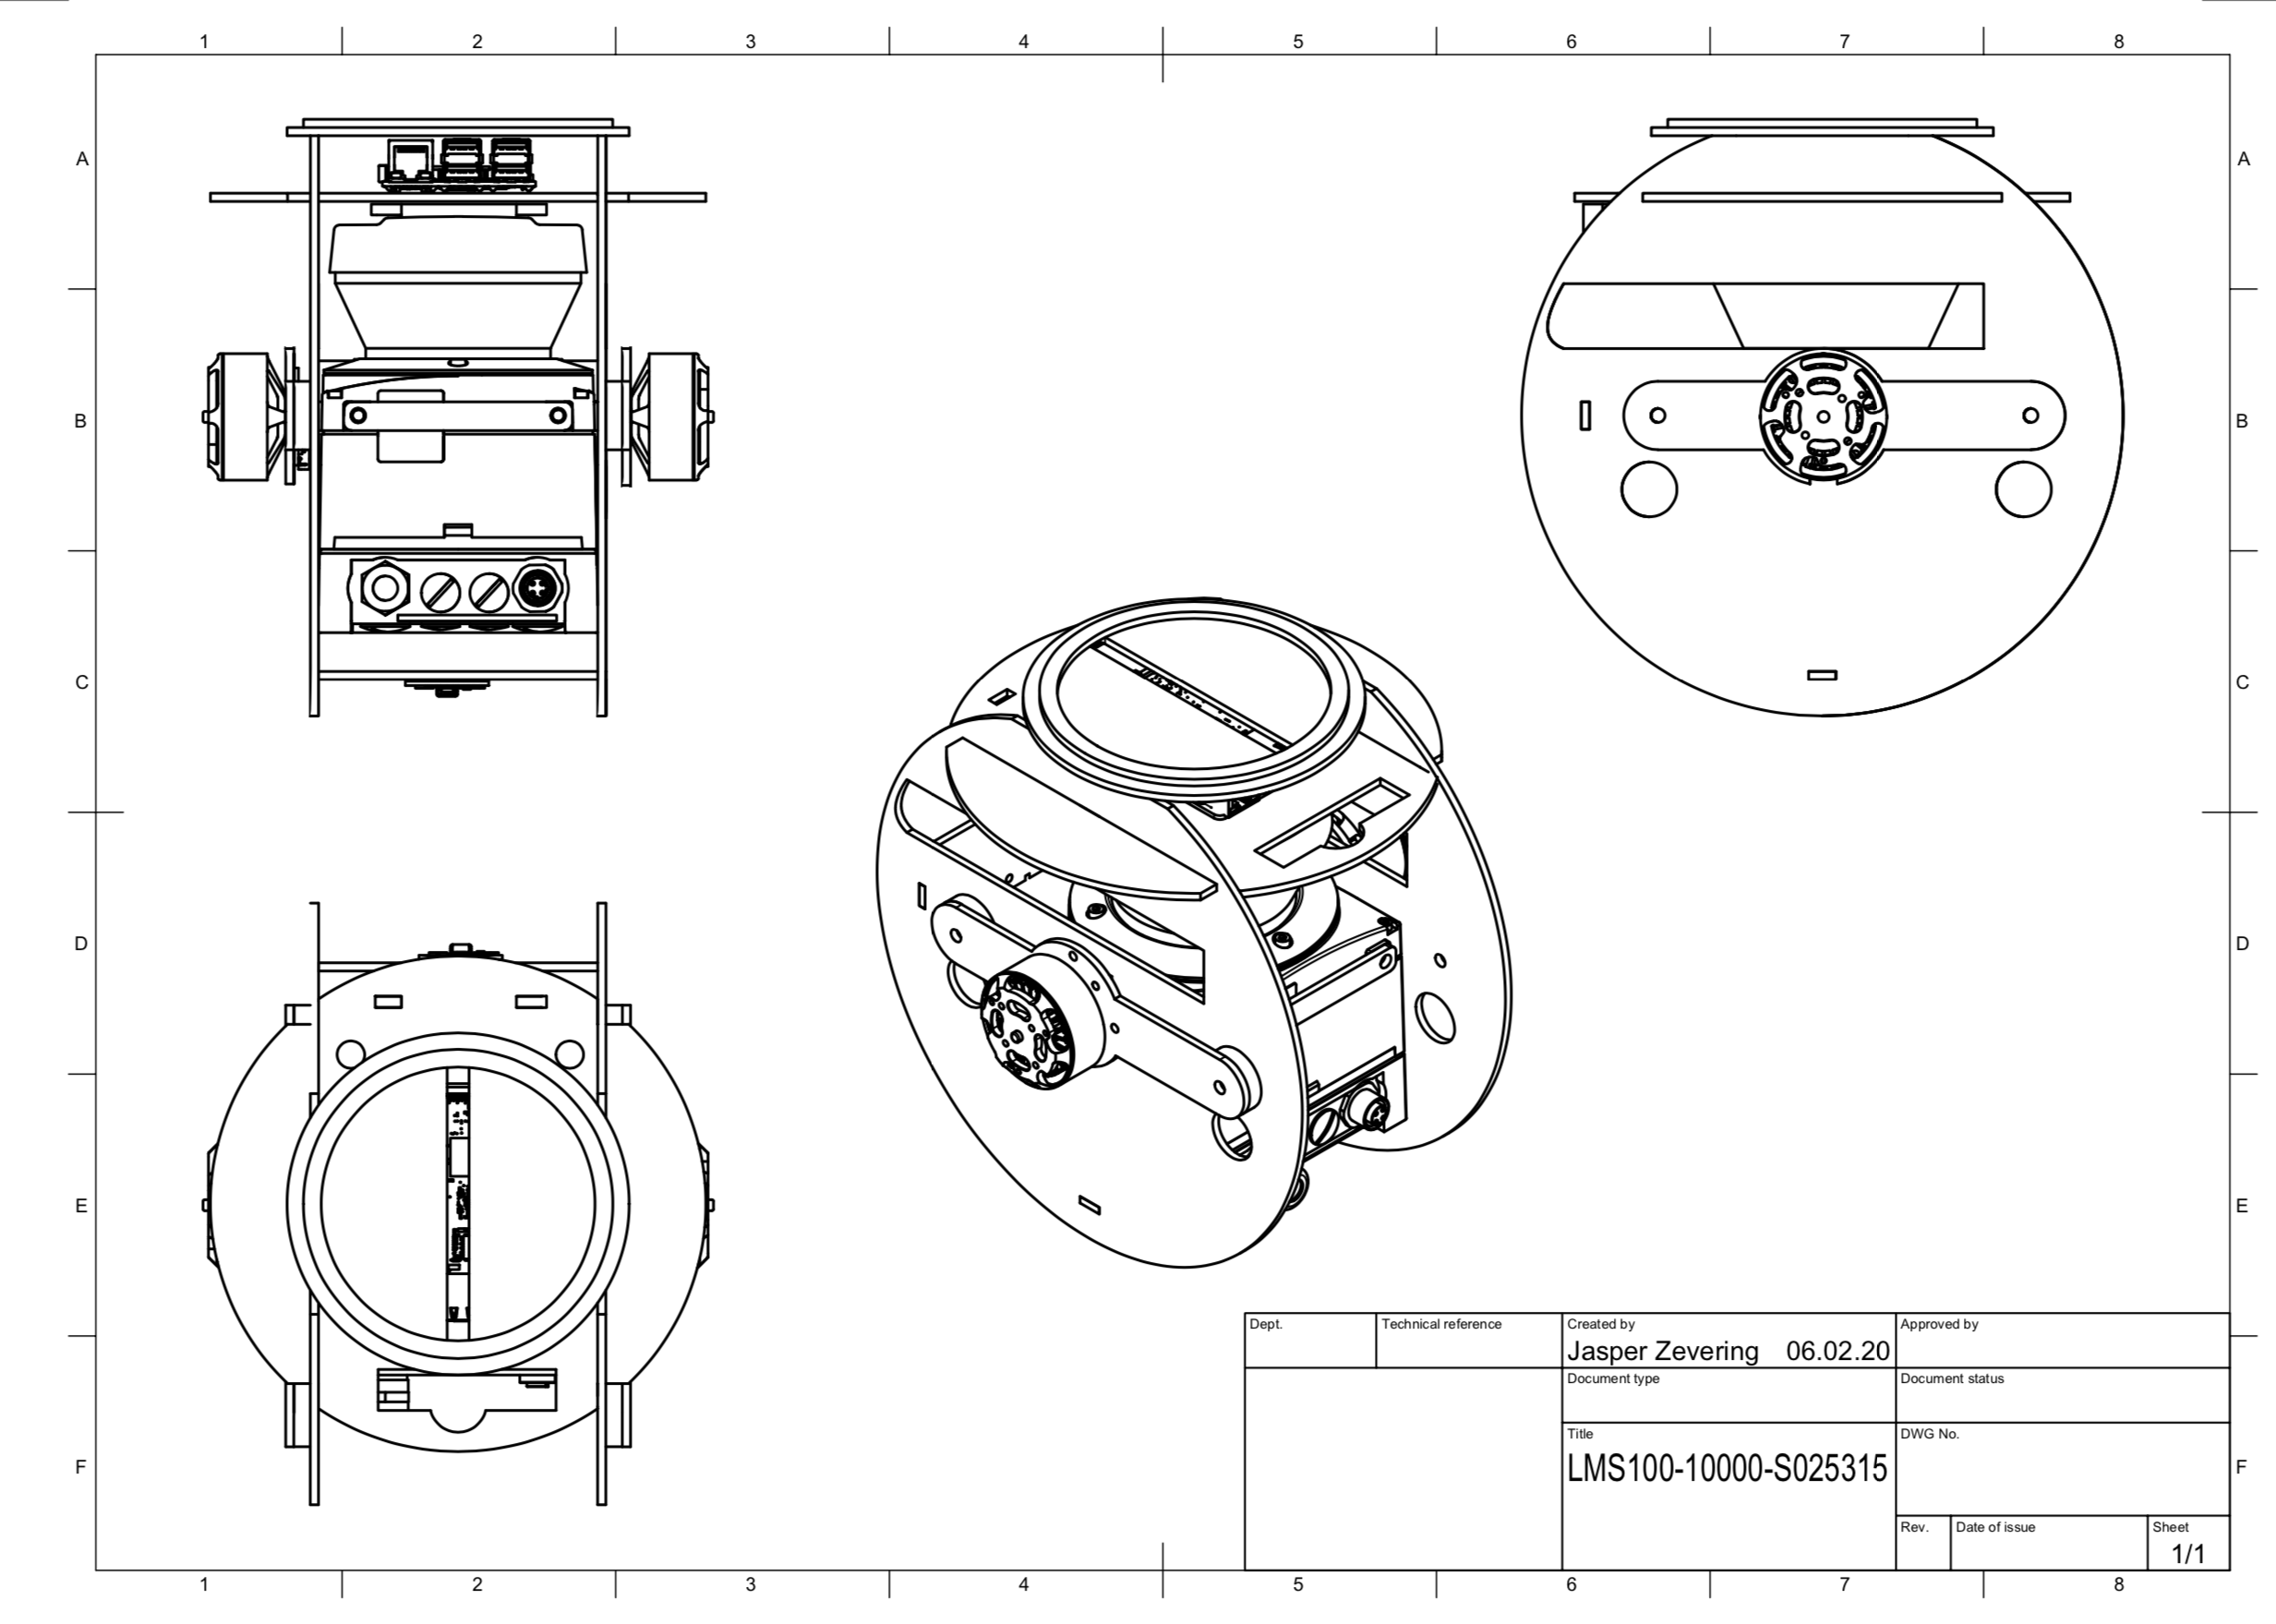
\includegraphics[width=\textwidth]{../Media/BlueprintPNG.png}                                                                                                                                                      
\caption{Blueprint of the mechanical structure of the spherical robot.}                                                                                                                                   
\label{sec:TechnicalApproach:fig:blueprint}                                                                                                                                                                       
\end{figure}                                                                                                                                                                                                      
                                                                                                                                                                                                                  
Figure \ref{sec:TechnicalApproach:fig:blueprint} shows a CAD blueprint of the overall interior layout of the mechanical structure of the L.U.N.A sphere, ignoring the outside sphere, flywheels and wiring.
The payload is mounted to supporting structural components which are made of acrylic glass.
The Raspberry Pi 3B boardcomputer is placed on top of the laser.
Above that, another supporting structure holds additional counterweights to correct for inhomogeneous weight distribution.                                                                                                     
The battery finds its place in front of the laser scanner on another supporting structure.
The two brushless motors were each placed on one side of the supporting structure with spacers that leave room for the side IMU underneath one of the motors.
Two other IMUs are placed in front of and beneath the laser to ensure coverage of all axes.                                                                                 

\begin{figure}                                                                                                                                                                                                    
\centering
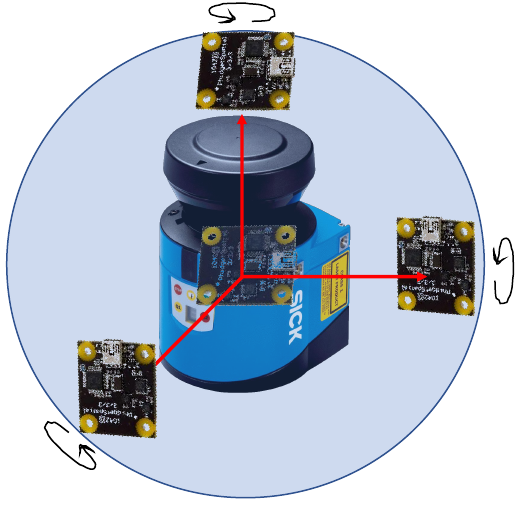
\includegraphics[width=0.5\textwidth]{../Media/virtualIMU.png}                                                                                                                                                      
\caption{Sketch that helps illustrate the combination of 3 IMUs into 1 virtual IMU that simulates being at the center of the sphere.}                                                                                                                           
\label{sec:SensorIntegration:fig:virtual}                                                                                                                                                                       
\end{figure}                                                                                                                                                                                                      

\subsection{Sensor Integration}
\label{sec:TechnicalApproach:sensorintegration}

The sensor integration is fully implemented with the Robot Operating System (ROS) using the Ubuntu distribution \href{http://wiki.ros.org/ROSberryPi}{ROSberryPi} which contains a pre-installed ROS version.
Overall, three seperate PhidgetsSpacial 10441B IMUs \cite{imuphidgets} keep track of the pose of the sphere.
Figure \ref{sec:SensorIntegration:fig:virtual} illustrates why three IMUs are used instead of just one.
\todo{Mehr erklären}
Previous prototypes have shown that transforming the data of only one non-centered IMU leads to lower quality measurements. \todo{die neue figure mit daten}
However, combining the measurements of three IMUs, where each of which measures only the static rotation around one of their rotational axes (which also represents a rotation axis of the sphere), leads to less noise.
Each IMU is perpendicular to the other two, so combining the axis measurements leads to a "virtual" IMU, which simulates being an IMU positioned at the center of the sphere. 

The IMUs also ship with accelerometers that are used to determine the full pose of the sphere.
Each IMU calculates their pose separately, using a quaternion extended Kalman filter (QEKF).
However, combining those poses into one does not have any positive effect, but only makes the software more resource demanding and slow.
Thus only the pose of the bottom IMU's accelerometer is used to keep track of the pose.

The motors are controlled using the piGPIO library. The GPIO signals are forwarded by the pins to two ESCs that drive the motors. 

Unfortunately, the brass weights are not drilled in the very center, causing an unbalance when rotating.
The resulting vibrations inhibit the movement of the sphere.
Thus a controller was implemented that measures the extend of the vibrations using standard deviations of the non-rotating axes of the IMU and adjusts the throttle of the motors accordingly.
This was done with a two-point controller with hysteresis.
Considering the translational velocity of the sphere in a controller is not possible.
The speed of the sphere is calculated by the rotational speed, which is why slippage of the sphere causes such a controller not to produce the desired motion. 

\subsection{Point Cloud Processing}                                                                                                                                                                                  
\label{sec:TechnicalApproach:pointcloudprocessing}
For the processing of the point cloud the 3D Toolkit (3DTK) was used.
This provides multiple methods and algorithms for processing 3D point clouds, especially the 6D continuous time Simultaneous Localization And Mapping (SLAM) algorithm (see \cite{3DARCH2017_1, LS2019}) as post-processing.
Therefore only the time-stamped raw data of the IMUs and laser-scanner is transferred and the estimation of the pose and the SLAM algorithm itself is performed externally.
For this prototype the transfer is realized using the host-function of ROS, giving the external PC the possibility to subscribe to the topics and process them.
3DTK itself takes pairs of files, one representing the pose, one the laser scanner data, and each file named by the time-stamp with an identifier if it is scan-data or pose.
Also, the use of USB-connected IMUs and ROS as transfer-mechanism of data leaves potential for enhancement and therefore reducing the load of the internal controller.

\section*{Results}
\label{sec:Results}

As proof of concept, the prototype of L.U.N.A sphere for 3D mapping using the concept impulse out of conservation of angular momentum as a unidirectional drive to roll a 2D laser scanner in an IMU equipped, pose-tracked spherical robot system, has been build and tested successfully. Potential for improvement and technical limitations have been identified.
The resulting sphere is shown in fig. \ref{sec:TechnicalApproach:fig:setup}
\begin{figure}
\centering                                                                                                                                                                                                        
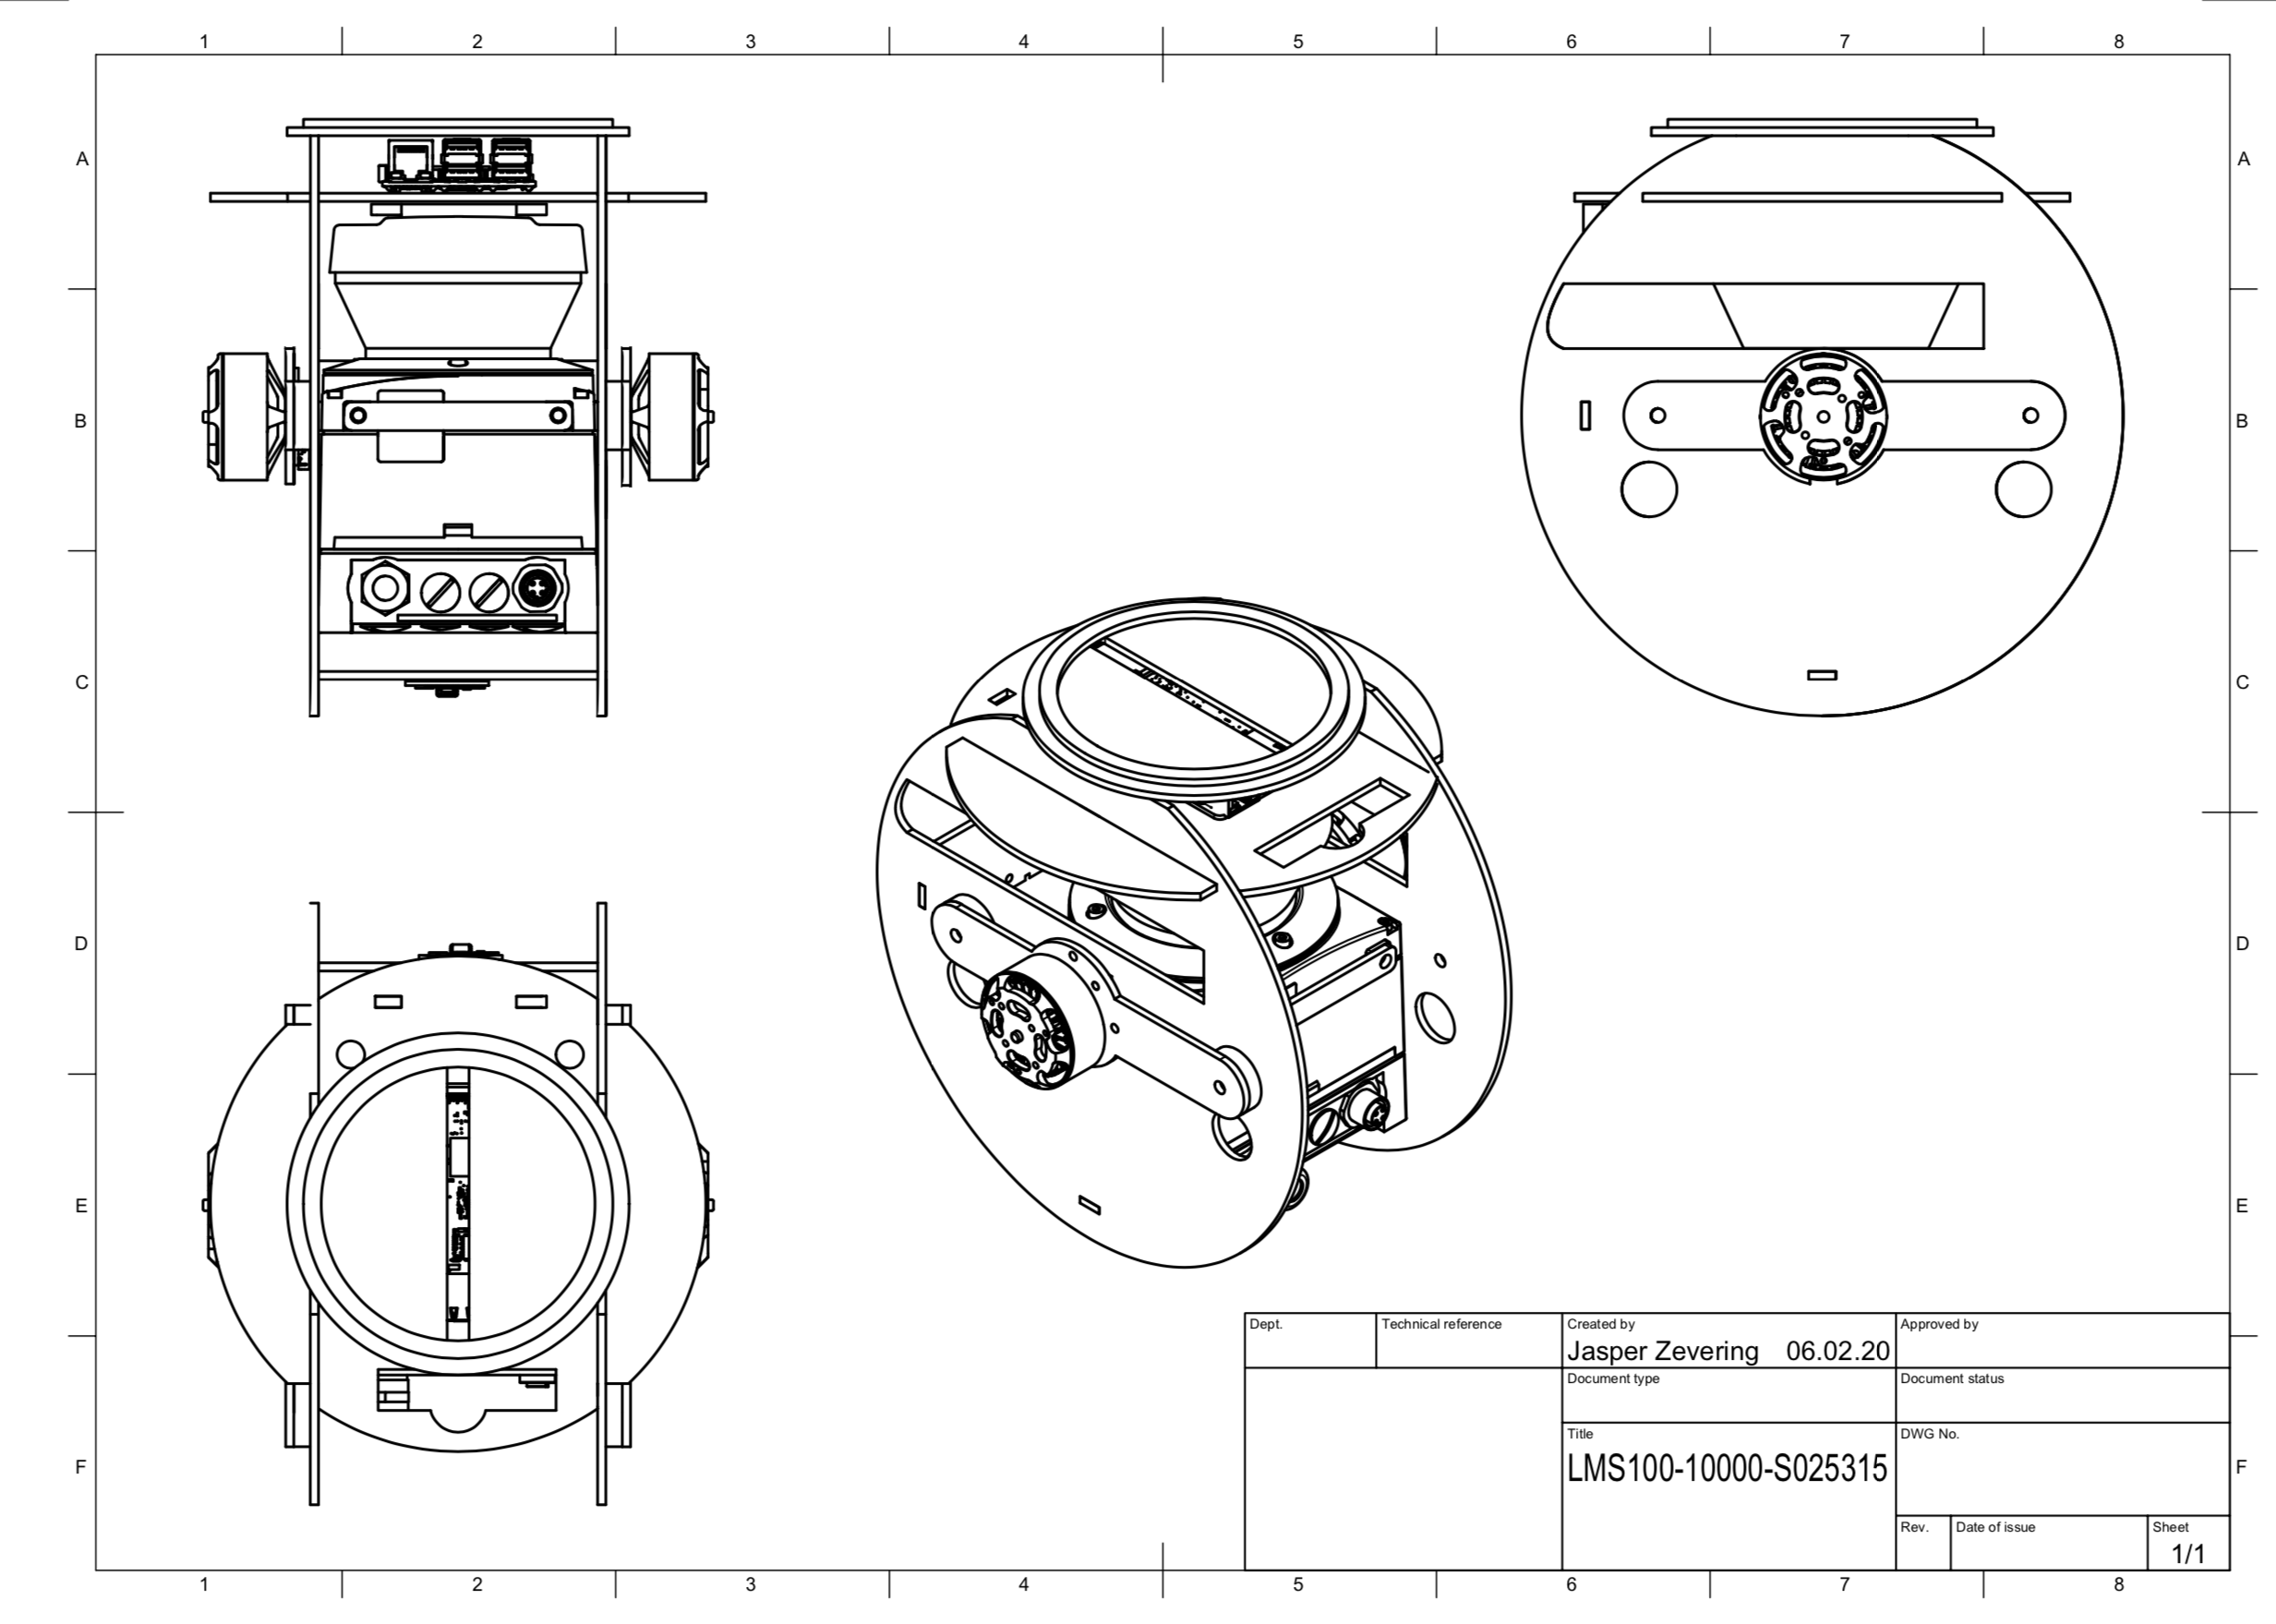
\includegraphics[height=50mm]{../Media/BlueprintPNG.png}                                                                                                                                                      \\
\vspace{0.5cm}
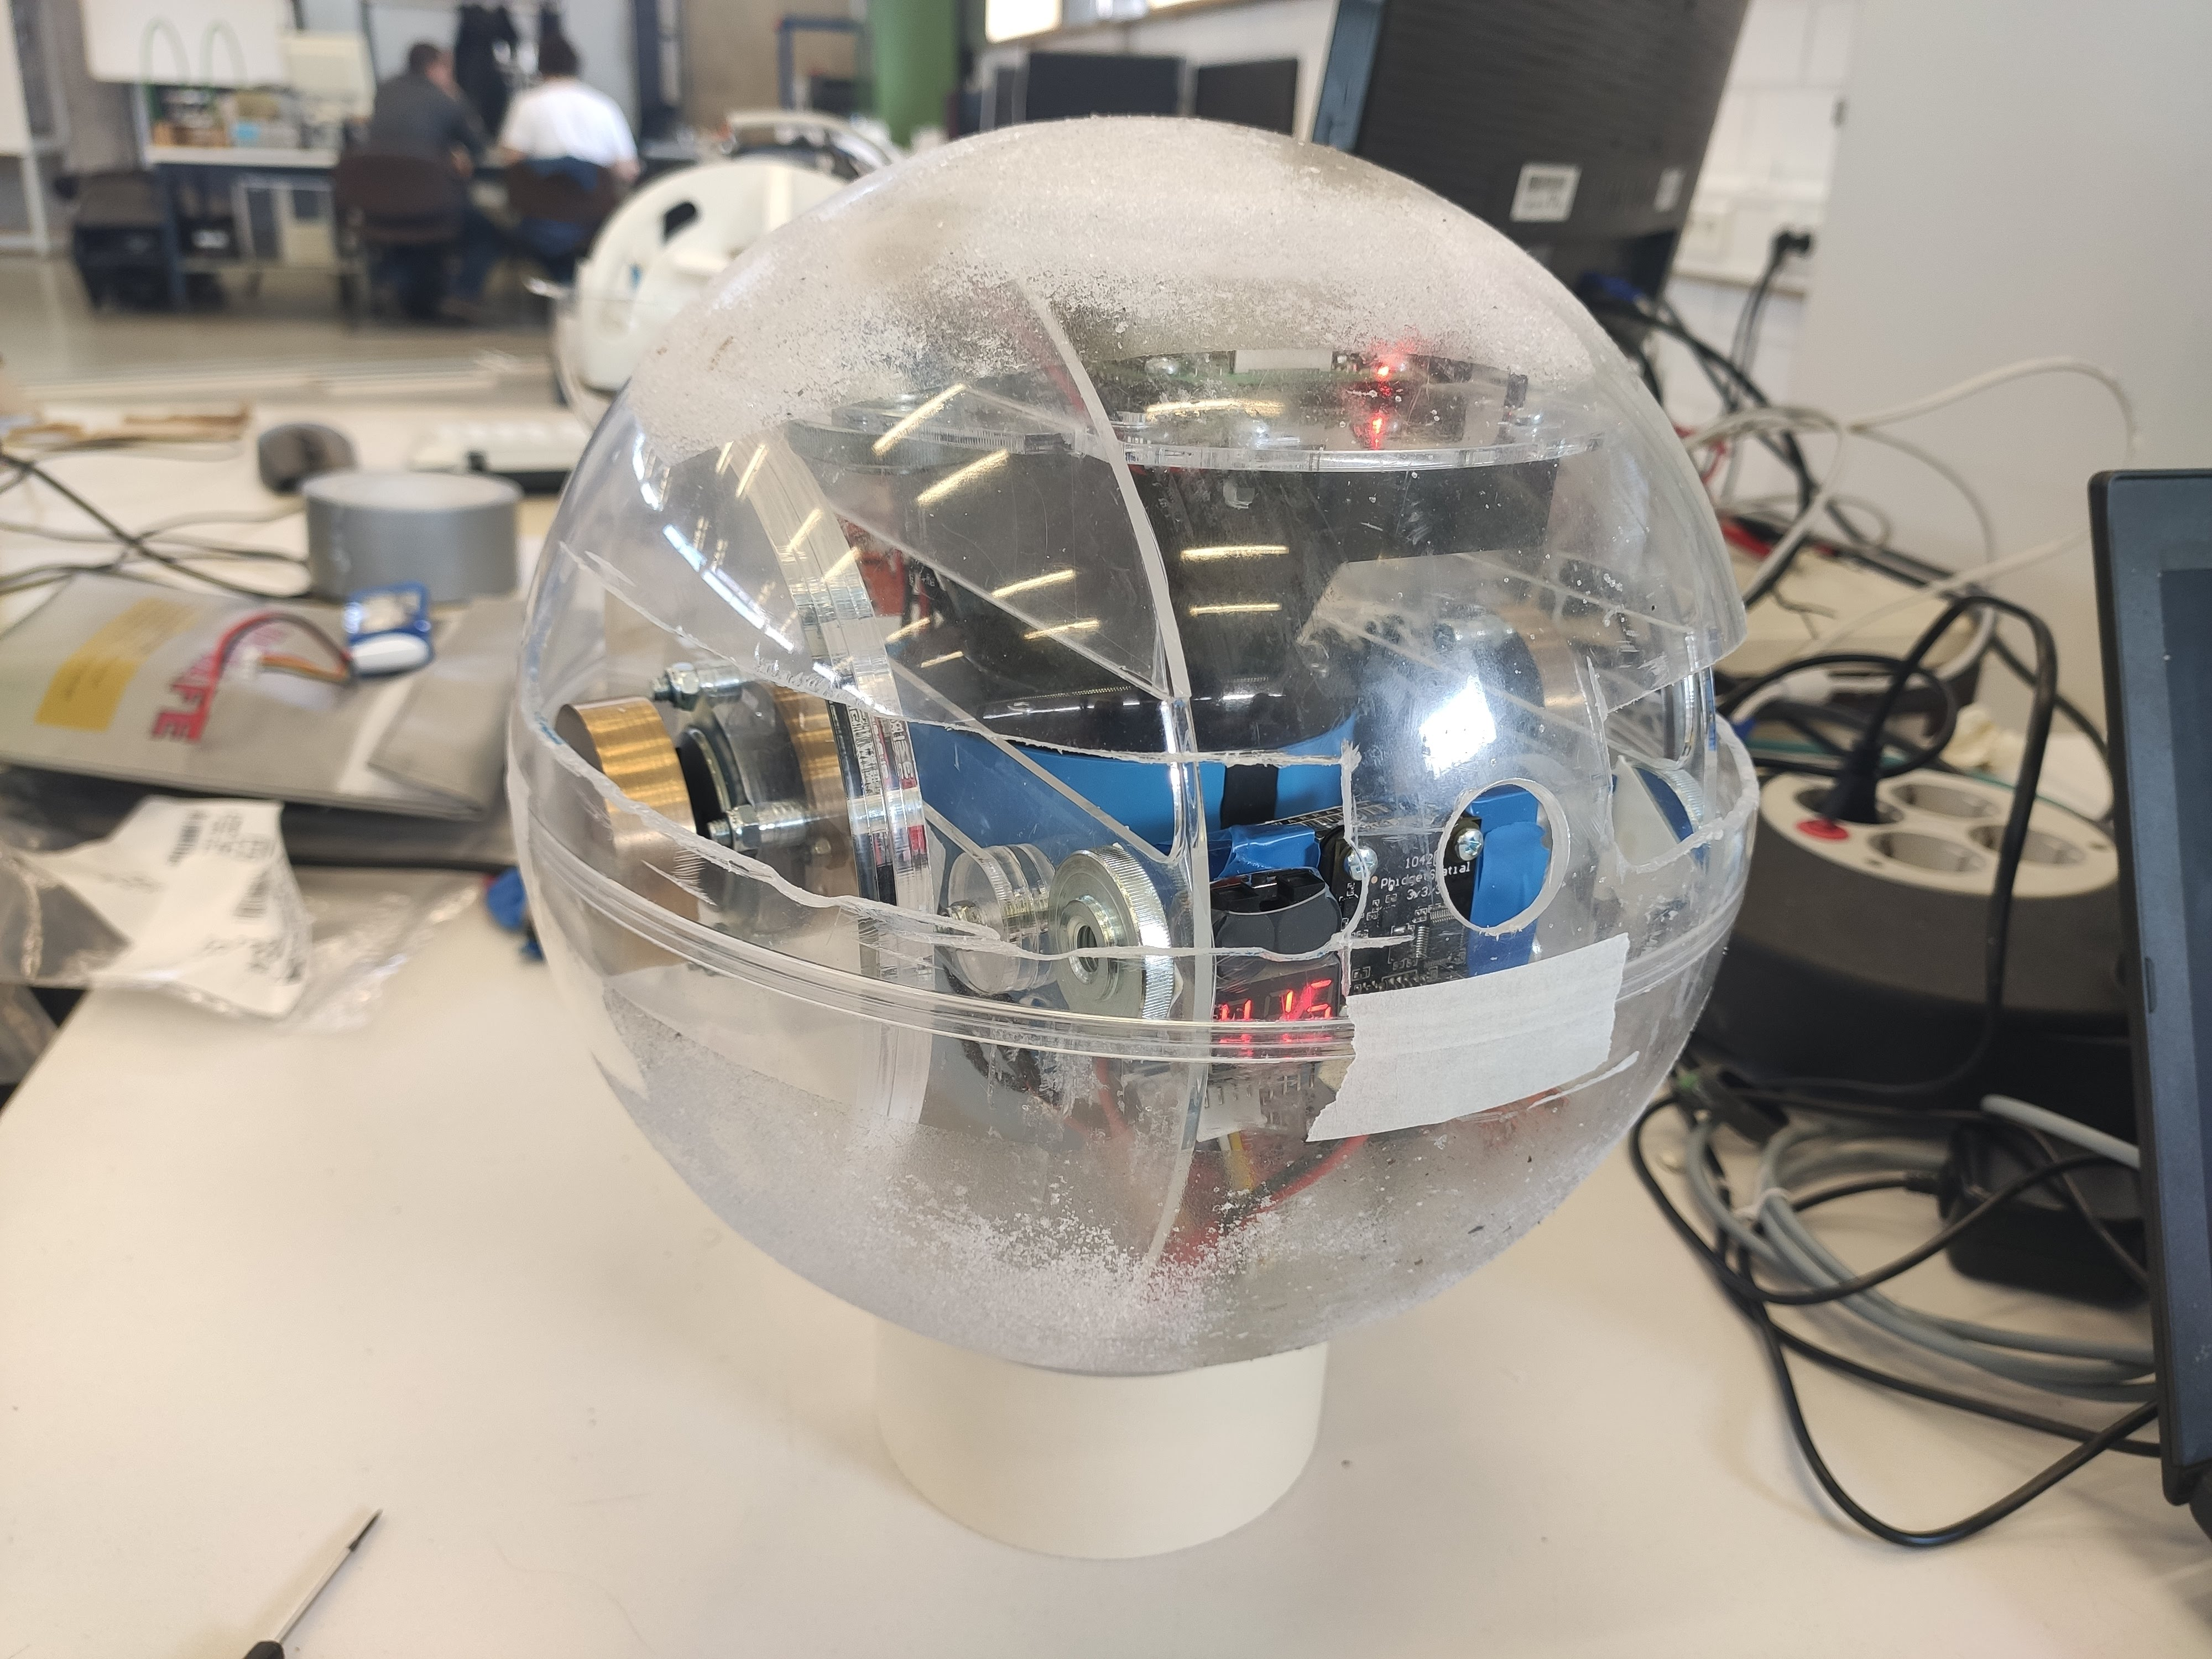
\includegraphics[height=50mm]{../Media/sphereFullshellLeft.jpg}
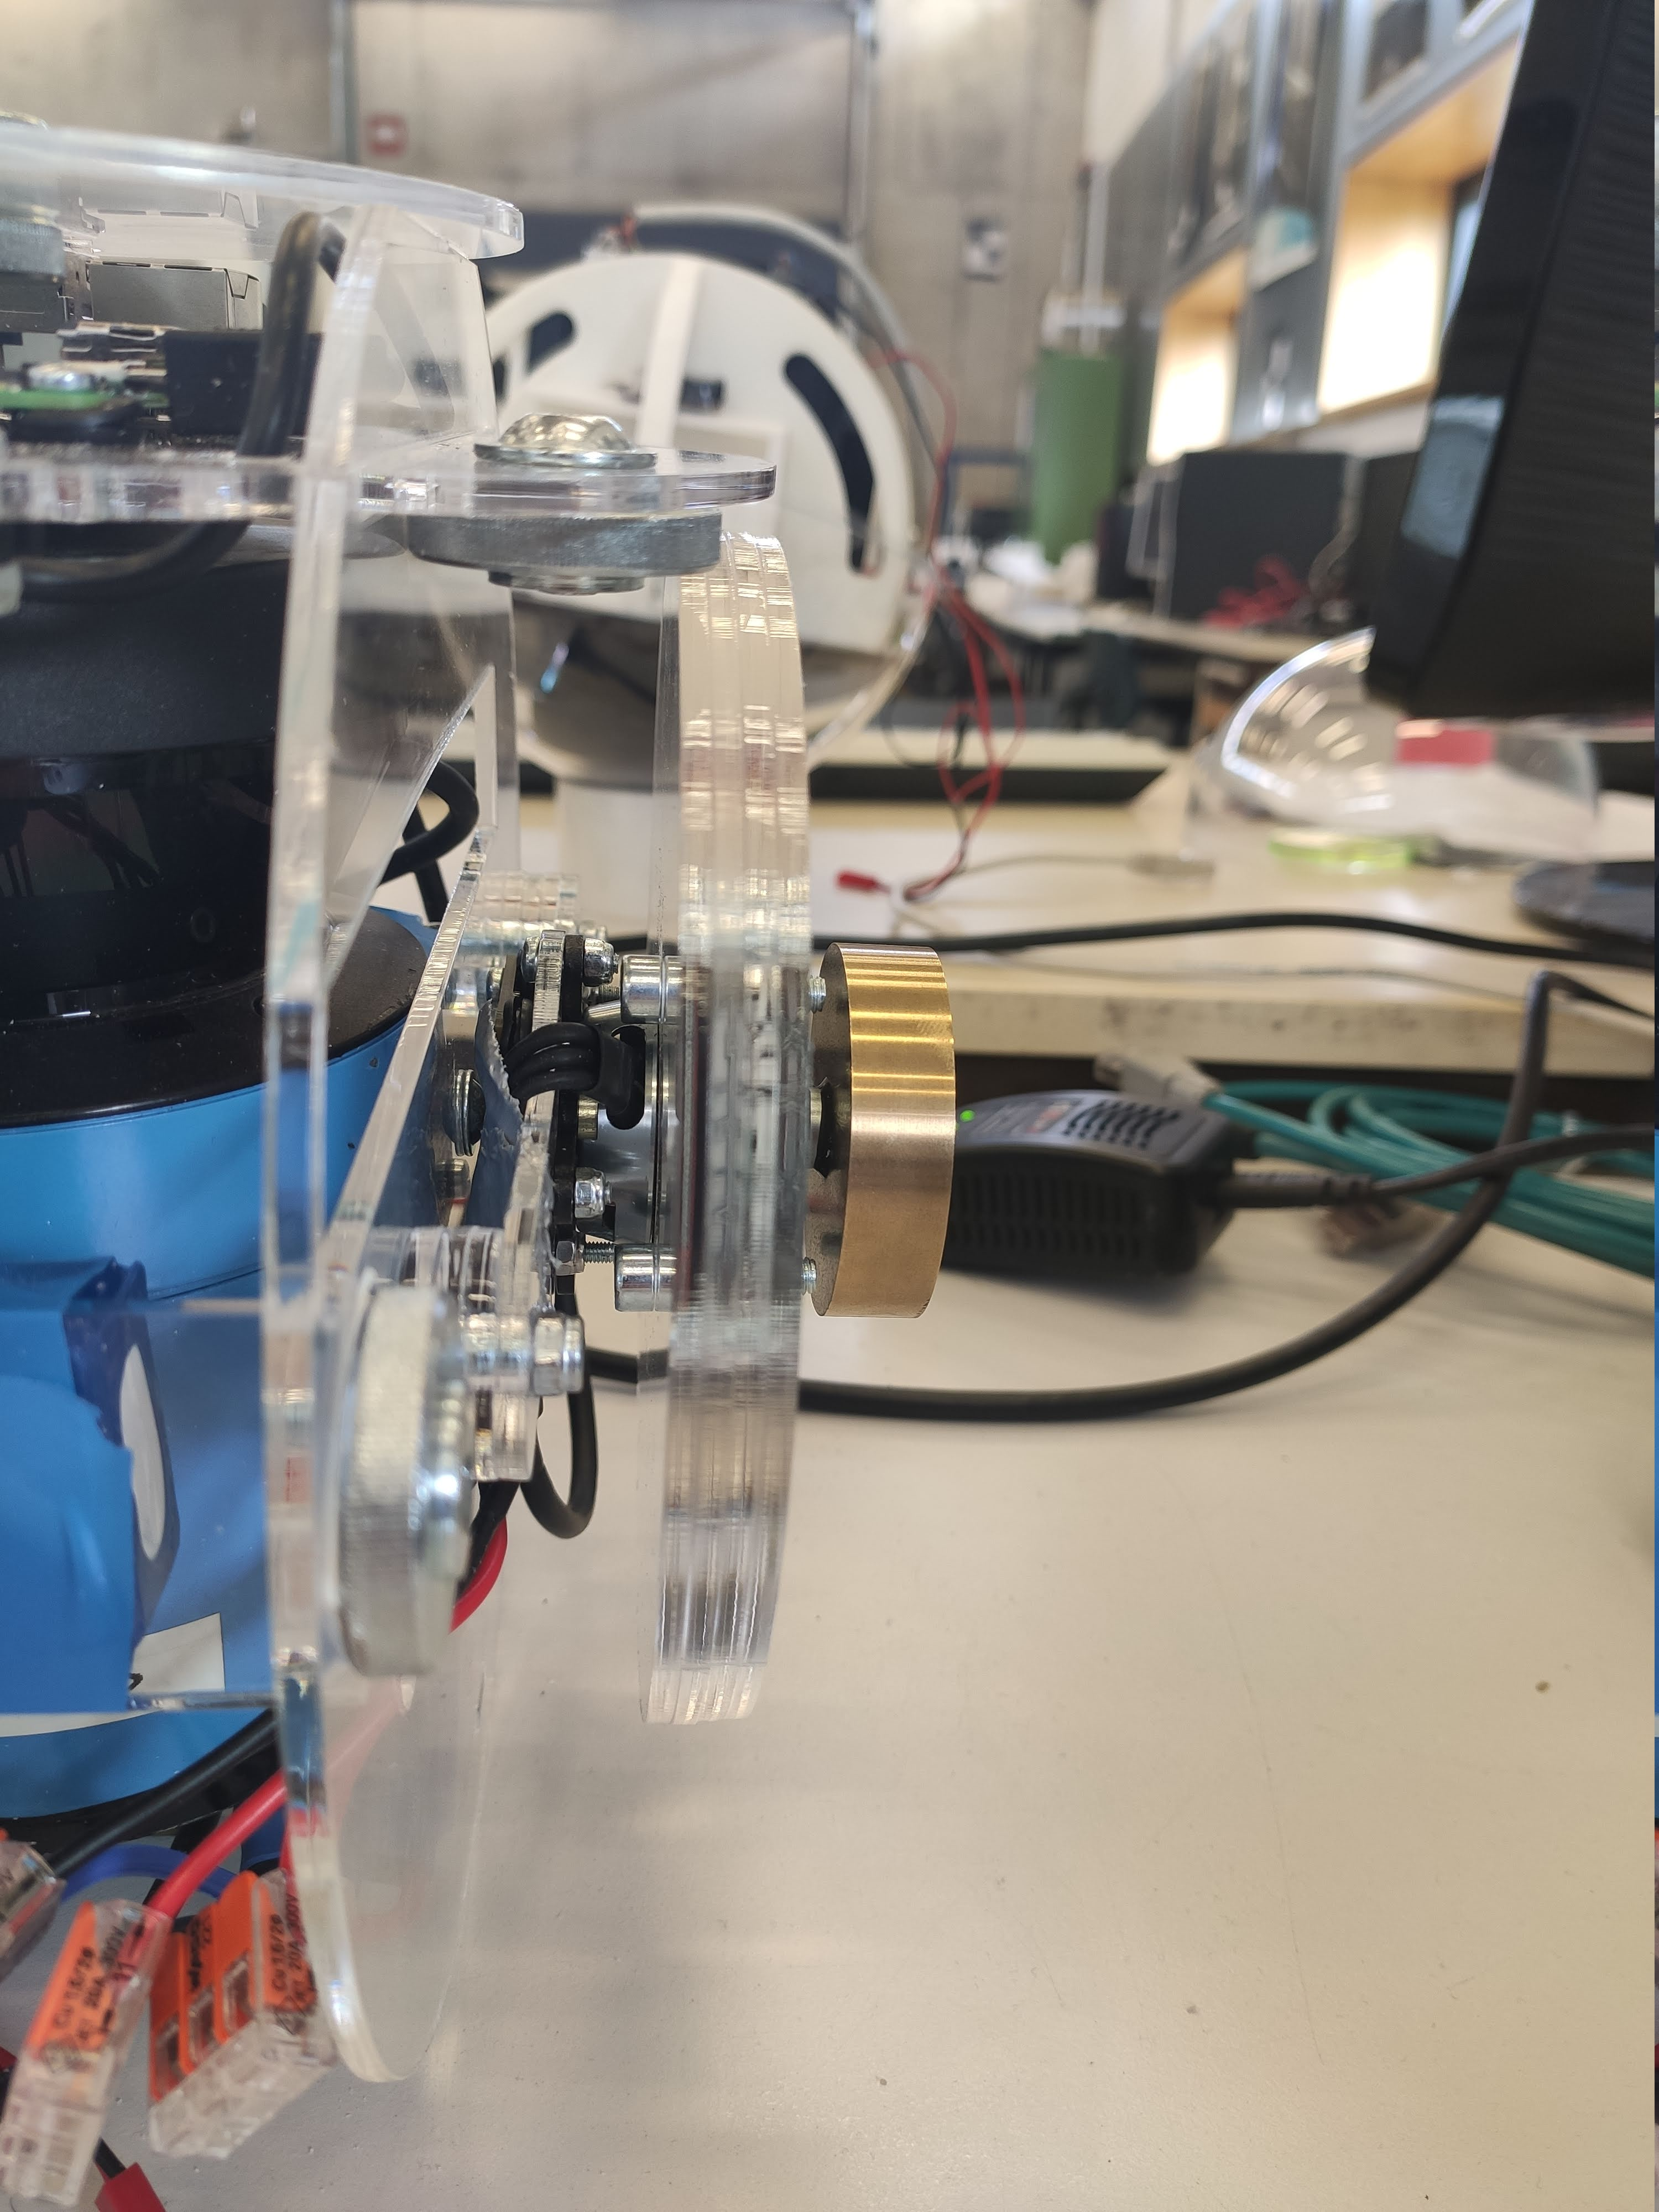
\includegraphics[height=50mm]{../Media/sphereRightMotor.jpg}   
\\\vspace{0.5cm}
\begin{subfigure}[b]{0.32\textwidth}
	\centering
	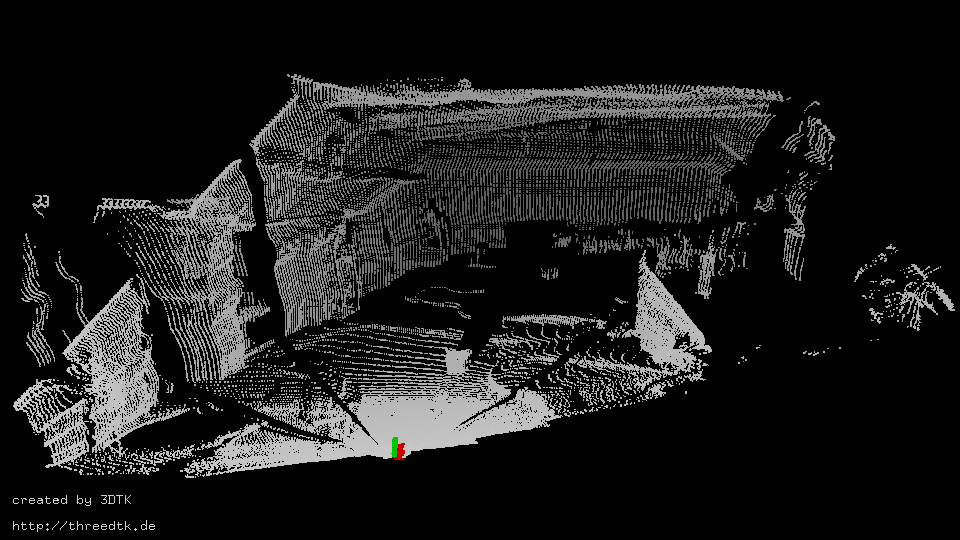
\includegraphics[width=\textwidth]{../Media/FirstDecentMap}
	\caption{Test with limited movement and no exterior shell.}
	\label{sec:experimentalResults:3DLaserScanning:fig:firstpointcloud}
\end{subfigure}
\begin{subfigure}[b]{0.32\textwidth}
	\centering
	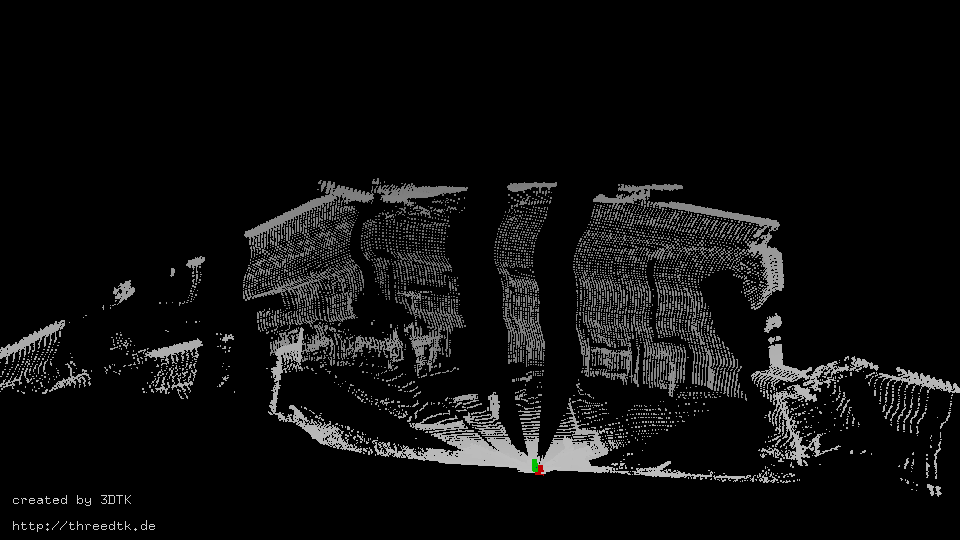
\includegraphics[width=\textwidth]{../Media/testScanWithTop}
	\caption{Test with limited movement and exterior shell.}
	\label{sec:experimentalResults:3DLaserScanning:fig:secondpointcloud}
\end{subfigure}
\begin{subfigure}[b]{0.32\textwidth}
	\centering
	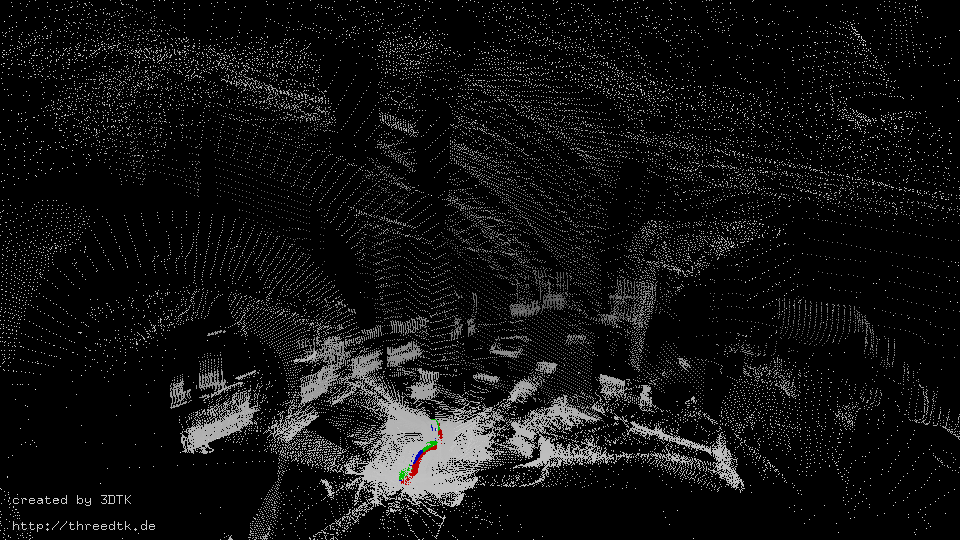
\includegraphics[width=\textwidth]{../Media/RollingTestMap}
	\caption{Test with exterior shell and full movement.}
	\label{sec:experimentalResults:3DLaserScanning:fig:thirdpointcloud}
\end{subfigure}
\caption{Hardware setup and laser-scanning Results of the L.U.N.A sphere prototype The Hardware including notches in the shell and friction granule (middle left). IMU (beneath supporting structure) and brushless motor  including flywheel mass (above supporting structure)(middle right).}
\label{sec:TechnicalApproach:fig:setup}

\end{figure}

\section{Conclusions}
\label{sec:conclusions}

In this paper a new cost efficient approach to 3D lase scanning was proposed: The L.U.N.A. sphere. It uses a 2D laser scanner mounted inside a spherical robot and uses the inherent rotational movement to form a radial scanning pattern and hence create a 3D point cloud. The spherical robot is based on conversation of angular momentum and uses flywheels to drive the robot forward. 

The prototype developed for the tests in this paper was able to move in one direction reliably on soft surfaces (such as rubber), however had difficulties with slippage on hard and slippery surfaces. In regards of 3D scanning this paper delivered a proof of concept, even though the result remain unsatisfactory as of right now. The biggest issues to overcome are reflections of the laser scanner beams by the exterior shell and synchronization issues between the IMU system and the laser scanner. 

Before the application of such a robot is possible more work is required. This could include improving the field of view of the laser scanner and extending the robot to two dimensional movement control. This would then enable autonomous mapping of environments using the L.U.N.A. sphere. 


\begin{acknowledgement}
The authors thank Dieter Ziegler.
\end{acknowledgement}

\bibliographystyle{plain}
\bibliography{andreas_publications}

\end{document}
